\subsection{Projektablauf}
Zur Zeit existiert bei allink auch kein offizieller Projektablauf. Ich bezeichne
den heutigen Zustand als ``natürliches Vorgehen''. Ein mögliches Projekt
kommt an einen Partner heran, entweder über eine Anfrage oder eine Akquisition,
er spricht sich wenn nötig mit den anderen Partner ab und nimmt dann die
Mitarbeiter mit in das Projekt, die er als nötig erachtet.

\subsubsection{Projektannahme und Offertenerstellung}
In der nachfolgenden Darstellungen \ref{pic:01_ist_prozesse_offerte_01} und
\ref{pic:01_ist_prozesse_offerte_02} ist der
aktuelle Prozess der Offertenerstellung ersichtlich. Die darin verwickelten
Akteuere sind der Kunde und der bzw. die Partner.

\begin{figure}[htbp]
\begin{center}
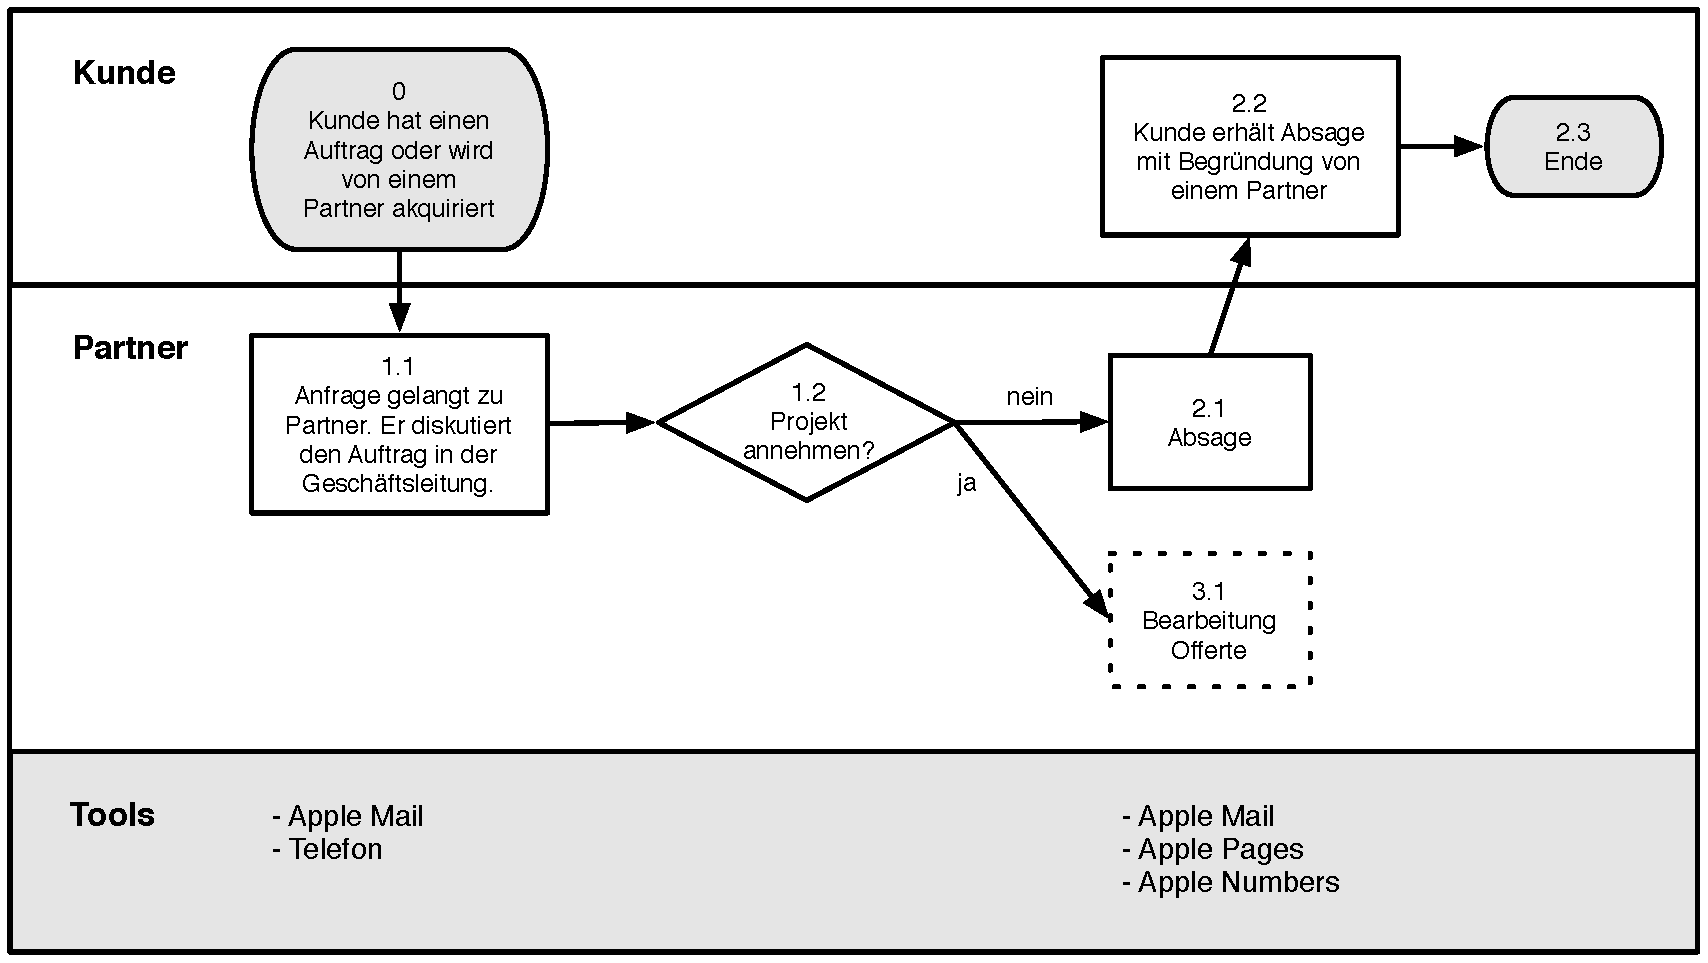
\includegraphics[width=0.99\textwidth,angle=0]{./bilder/01_ist_prozesse_offerte_01.pdf}
\caption{Offertenerstellungs Prozess von allink März 2011 1/2}
\label{pic:01_ist_prozesse_offerte_01}
\end{center}
\end{figure}

\paragraph{0}
Als Start eines Projektablaufes wird entweder ein neues Projekt akquiriert, 
durch einen Pitch oder eine normale Anfrage, oder ein Kunde kommt mit einem
Projekt auf uns zu.

\paragraph{1.1}
Die Projekte gelangen zur Zeit immer als erstes zu einem Partner. Sehr selten
bringt ein Mitarbeiter durch einen seiner Kontakte ein Projekt ein. Aber auch in
diesem Fall, würde es als erstes an einen Partner herangetragen.
Er diskutiert den möglichen Auftrag mit den anderen Partnern in der Geschäftsleitung.
Diese entscheide demokratisch ob ein Projekt angenommen oder abgelehnt wird. 
Sofern nicht alle Partner anwesend sein können, haben die anderen Partner
die Kompetenz, alleine zu entscheiden.

\paragraph{2.1}
Im Falle einer Absage tritt ein Partner wieder mit dem Kunden in Kontakt.
In den meisten Fällen natürlich der Partner, der bereits mit dem Kunden Kontakt
hatte.

\paragraph{2.2}
Dem Kunden wird erklärt, aus welchen Gründen das Projekt nicht angenommen
und durchgeführt werden kann.

\begin{figure}[htbp]
\begin{center}
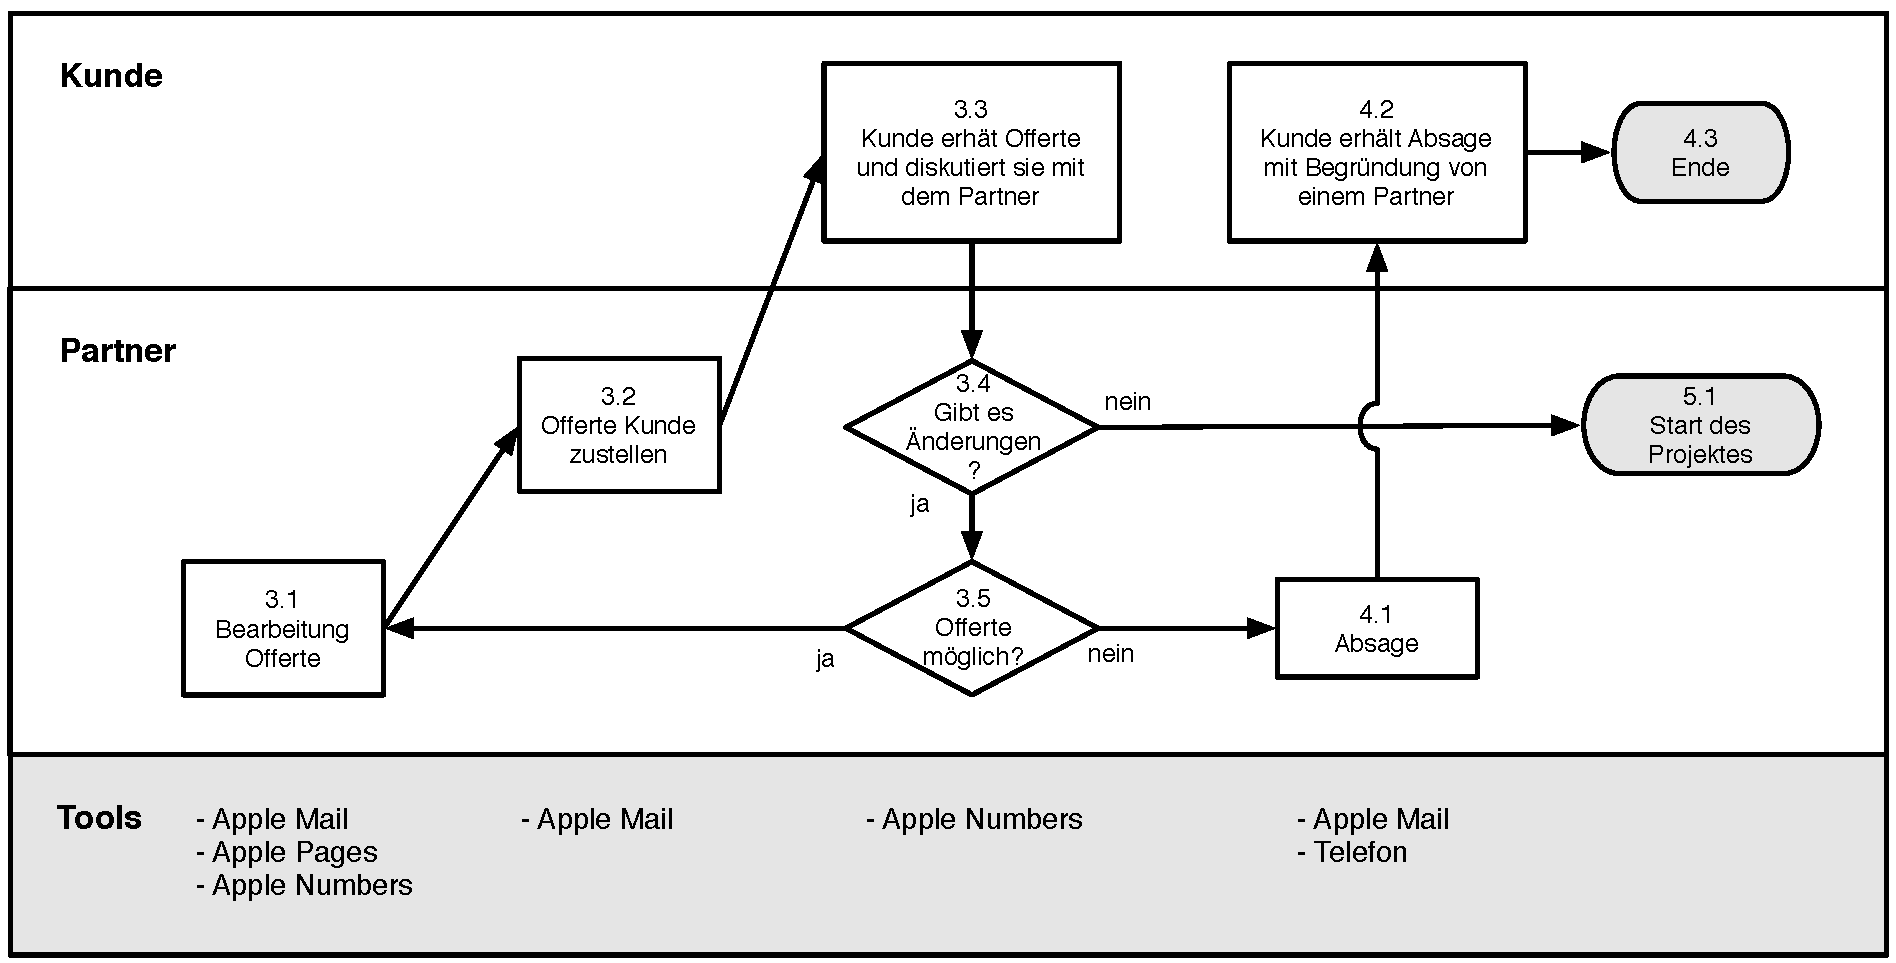
\includegraphics[width=0.99\textwidth,angle=0]{./bilder/01_ist_prozesse_offerte_02.pdf}
\caption{Offertenerstellungs Prozess von allink März 2011 2/2}
\label{pic:01_ist_prozesse_offerte_02}
\end{center}
\end{figure}

\paragraph{3.1}
Sollte das Projekt angenommen werden, wird auf Grund den zu erbringenden
Dienstleistungen eine möglichst genaue Offerte erstellt. Diese Schätzungen
basieren meist auf Erfahrungswerten aus anderen Projekten.

\paragraph{3.2}
Die Offerte wird dann dem Kunden zugestellt. In vielen Fällen wird dem Kunden
die Offerte präsentiert und genauer erklärt.

\paragraph{3.3}
Der Kunde diskutiert dann mit dem oder den Partnern die Offerte und bringt
bei bedarf Änderungen und Wünsche an.

\paragraph{4.1}
Kann man sich mit dem Kunden nicht einigen, also wünscht der Kunde Änderungen
an der Offerte oder den zu erbringenden Dienstleistungen, die von unserer Seite
nicht mehr möglich sind, muss das Projekt abgesagt werden.

\paragraph{4.2}
Dem Kunden wird erklärt, aus welchen Gründen die Offerte nicht angepasst oder
die Dienstleistung nicht erbringt werden kann.

\paragraph{5.1}
Im Falle einer Einigung und einer Auftragserteilung startet das eigentliche
Projekt.

Die Anfrage endet entweder in einer Absage oder einem Start eines neuen 
Projektes. Wenn das Projekt nicht zustande kommt, werden die Aufwände der
Akquisition und der Offertenerstellung zurzeit vernachlässigt und somit von
den übrigen Projekten getragen.

\subsubsection{Projektdurchführung}
Einleitungstext...

\begin{figure}[htbp]
\begin{center}
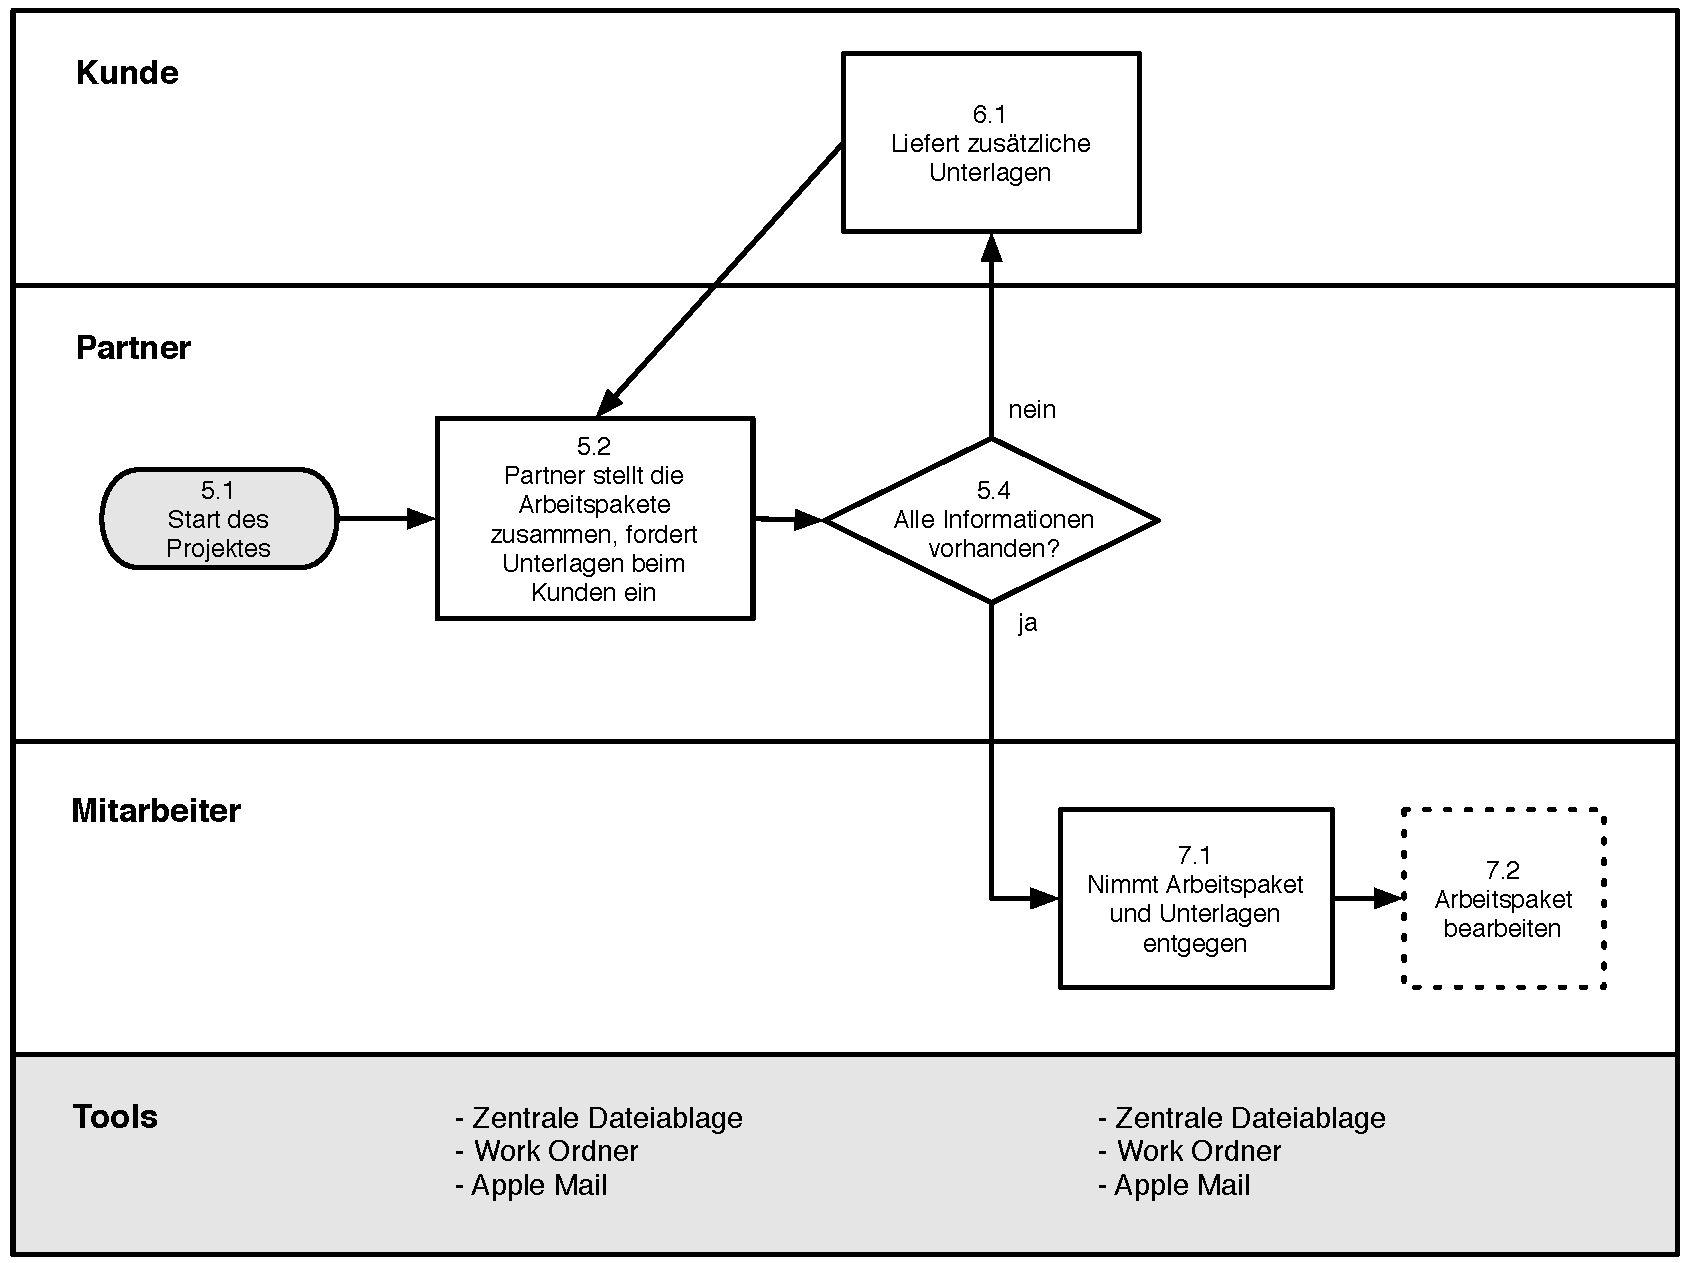
\includegraphics[width=0.99\textwidth,angle=0]{./bilder/02_ist_prozesse_arbeit_01.pdf}
\caption{Projektumsetzungs Prozess von allink März 2011 1/2}
\label{pic:02_ist_prozesse_arbeit_01}
\end{center}
\end{figure}

\begin{figure}[htbp]
\begin{center}
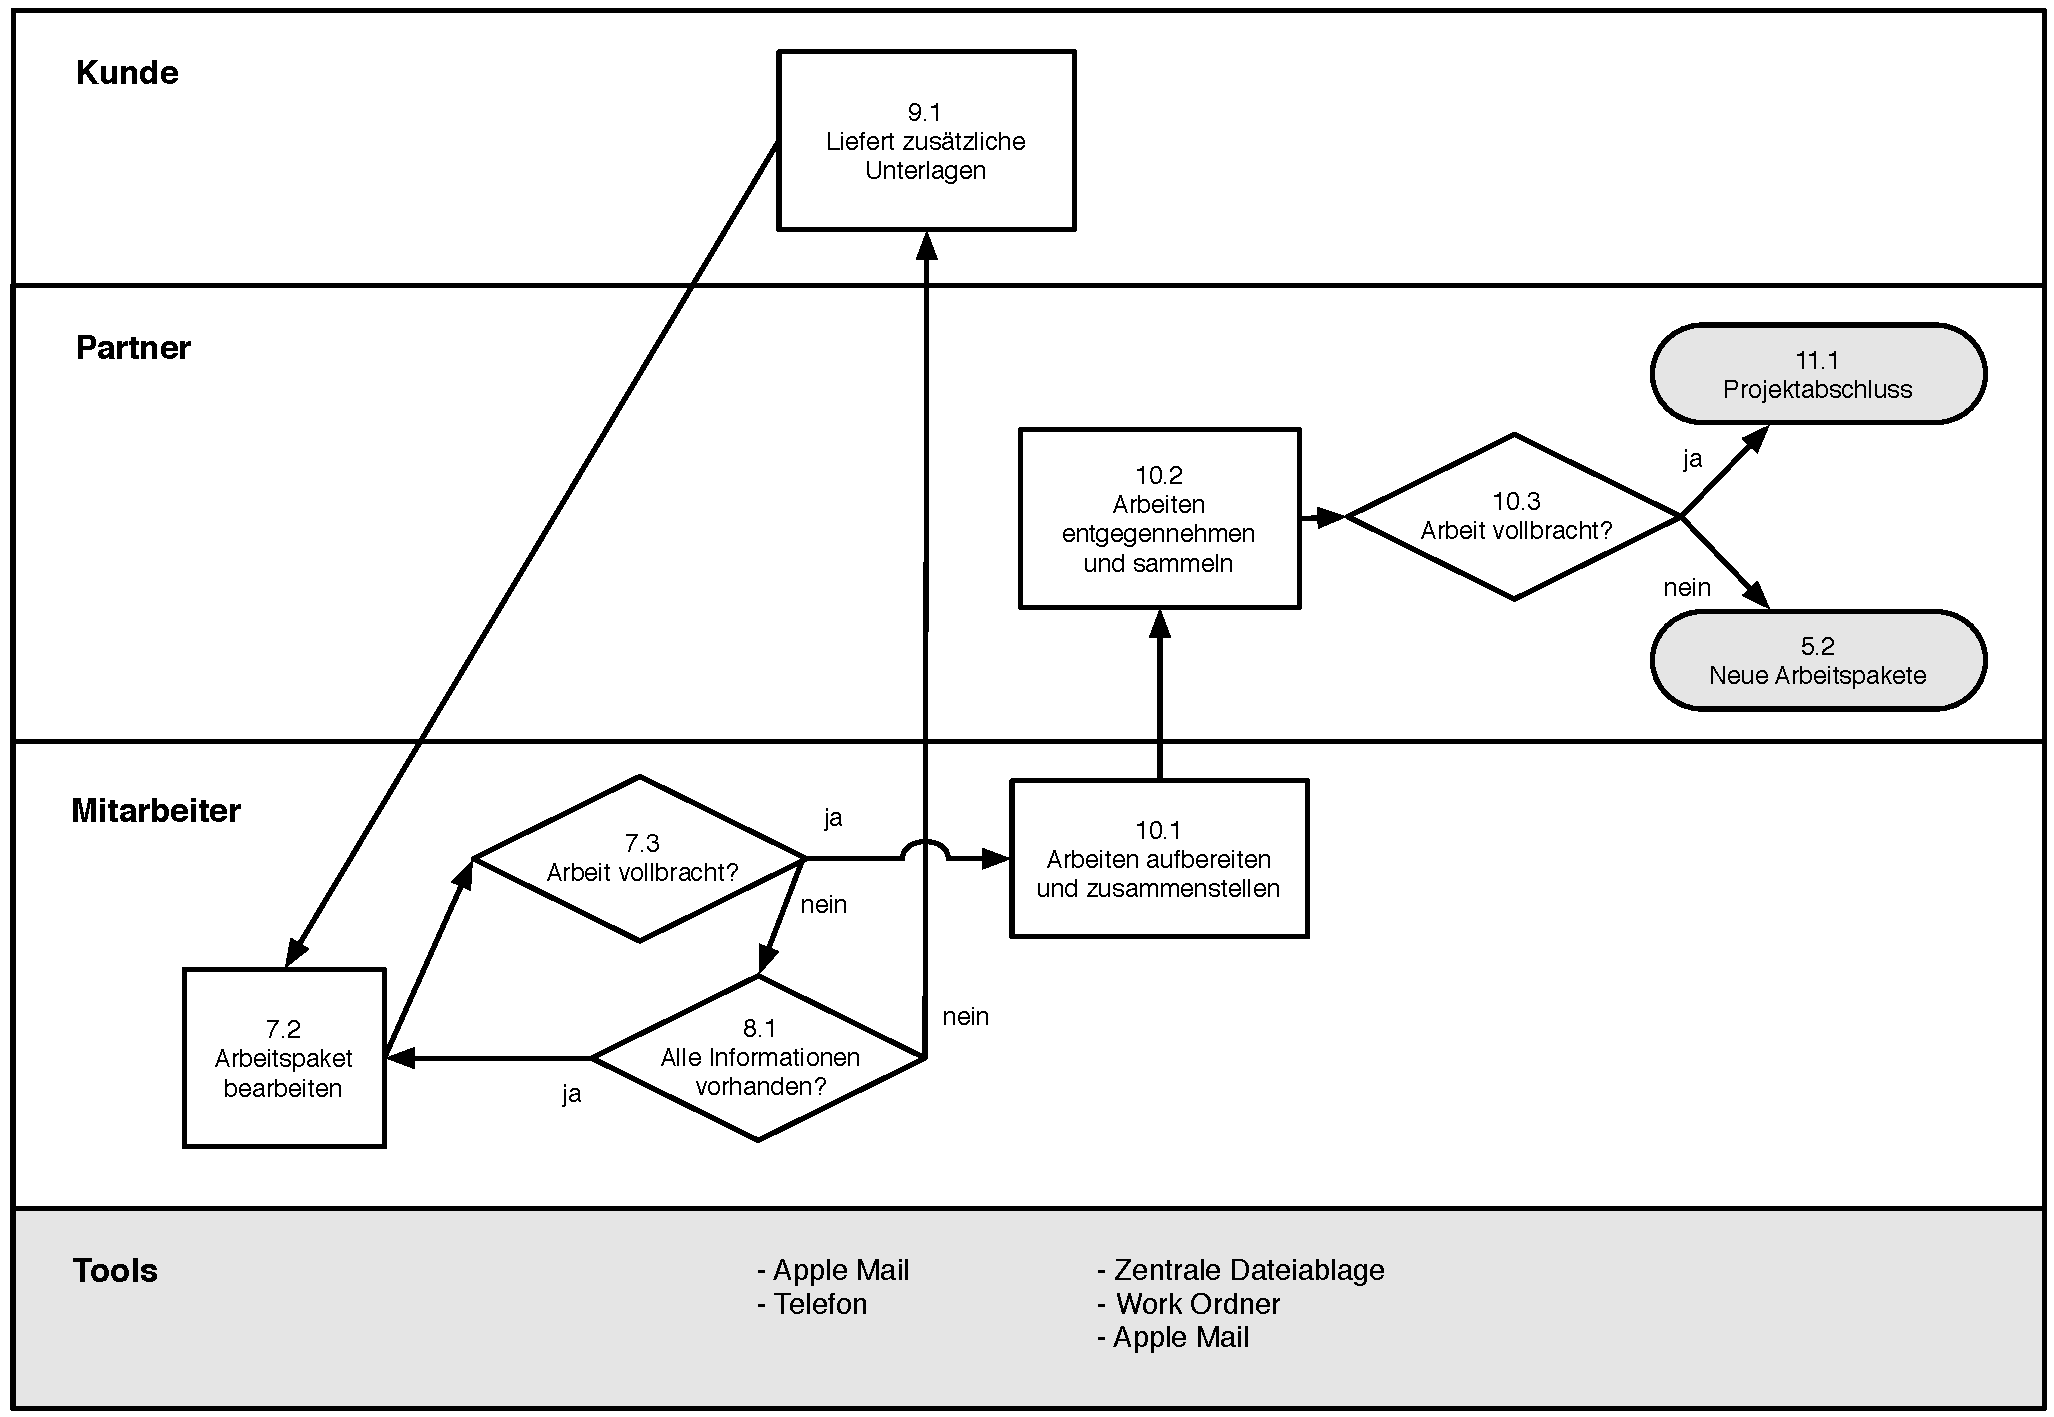
\includegraphics[width=0.99\textwidth,angle=0]{./bilder/02_ist_prozesse_arbeit_02.pdf}
\caption{Projektumsetzungs Prozess von allink März 2011 2/2}
\label{pic:02_ist_prozesse_arbeit_02}
\end{center}
\end{figure}

Detaillierte Beschreibung des Prozesses...

\subsubsection{Projektabschluss}
Einleitungstext...

\begin{figure}[htbp]
\begin{center}
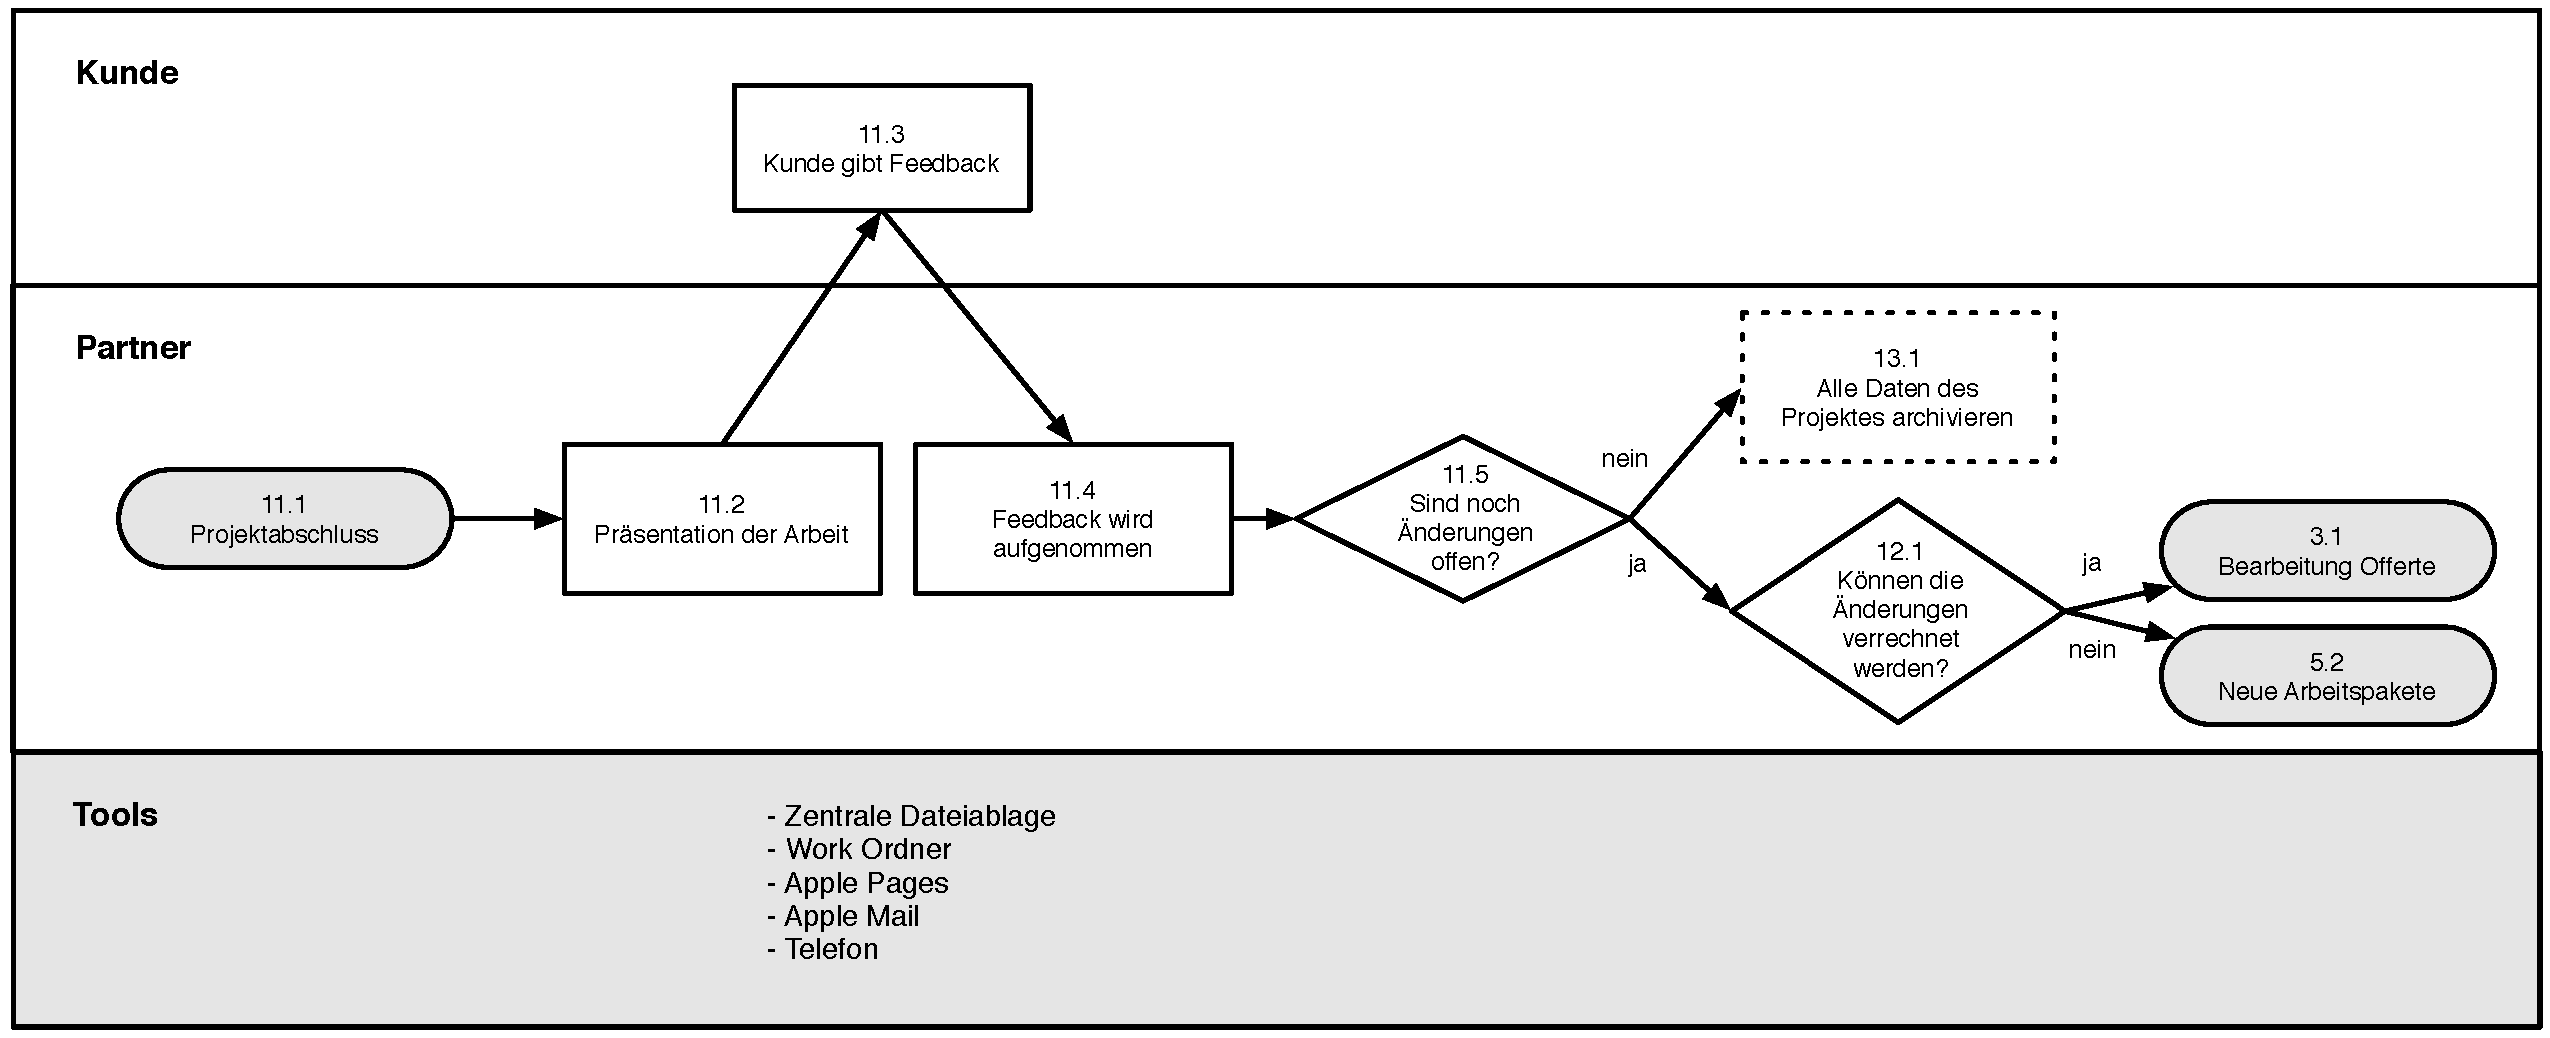
\includegraphics[width=0.99\textwidth,angle=0]{./bilder/03_ist_prozesse_abschluss_01.pdf}
\caption{Projektabschluss Prozess von allink März 2011 1/2}
\label{pic:03_ist_prozesse_abschluss_01}
\end{center}
\end{figure}

\begin{figure}[htbp]
\begin{center}
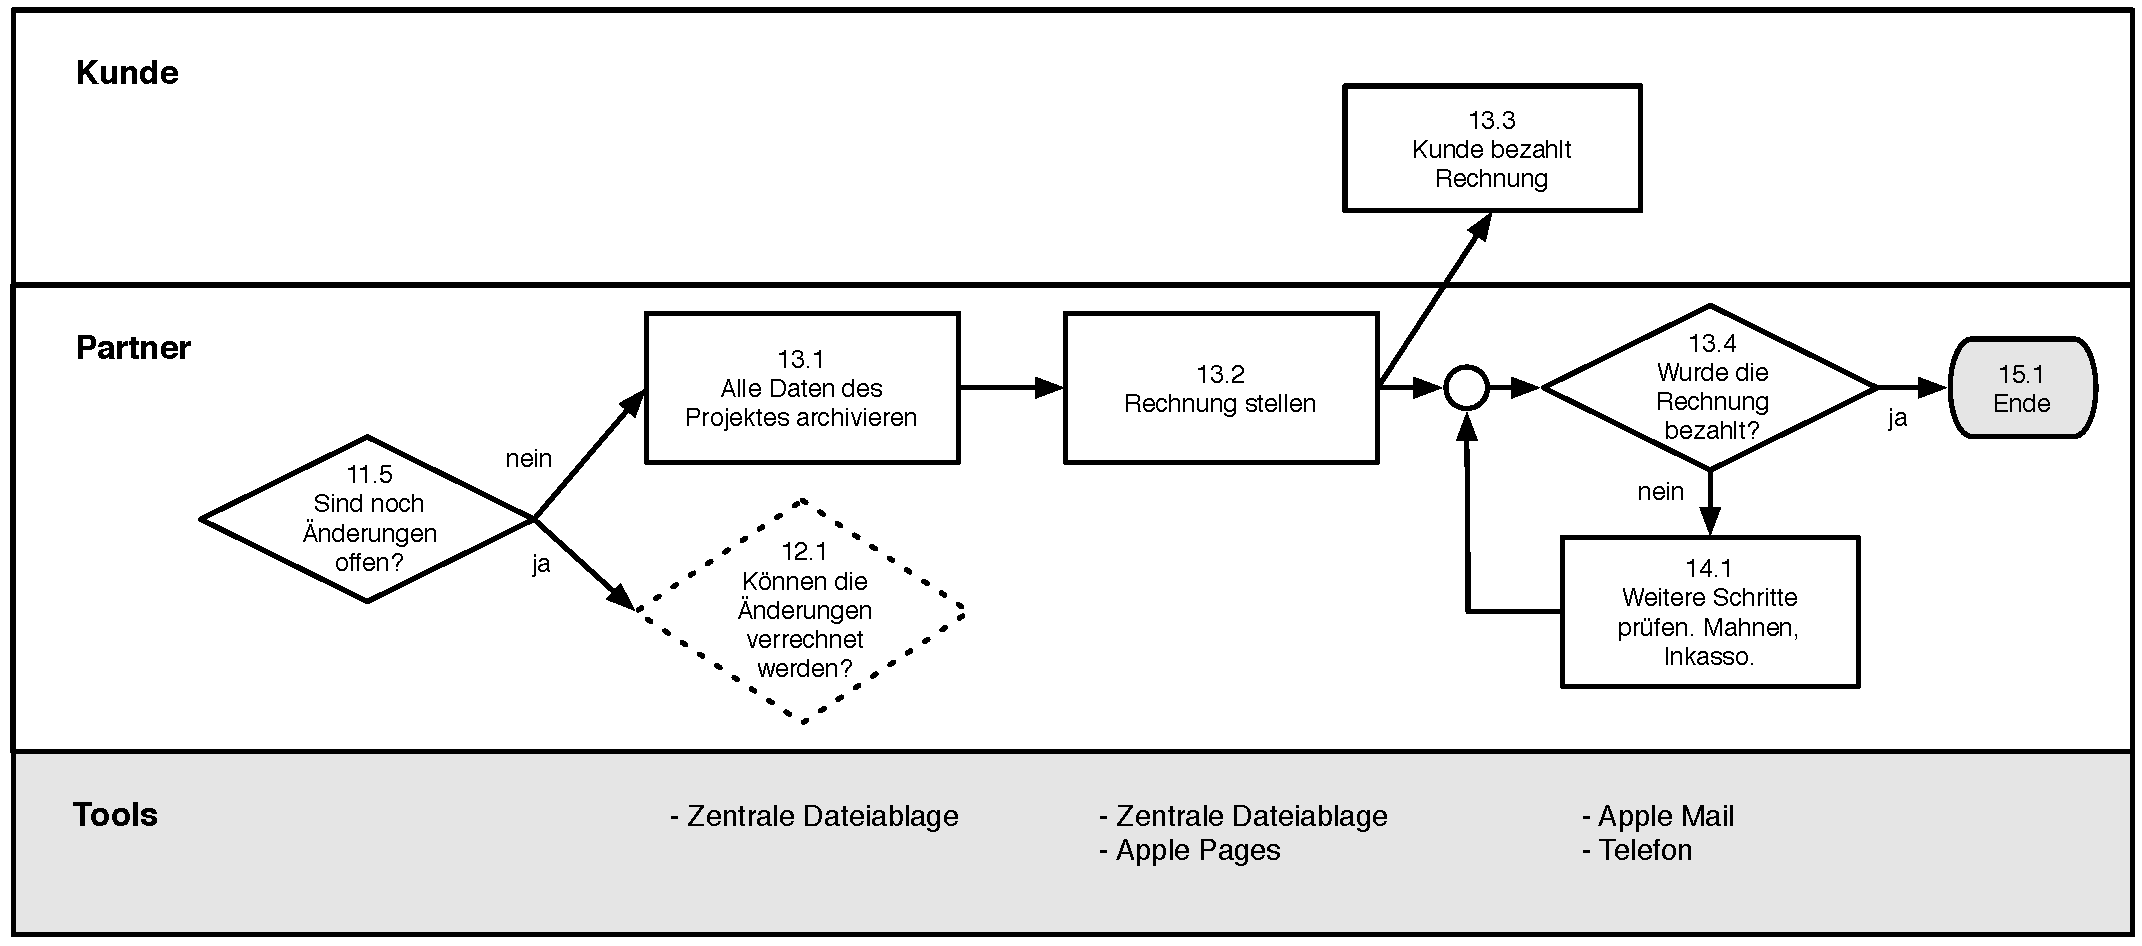
\includegraphics[width=0.99\textwidth,angle=0]{./bilder/03_ist_prozesse_abschluss_02.pdf}
\caption{Projektabschluss Prozess von allink März 2011 2/2}
\label{pic:03_ist_prozesse_abschluss_02}
\end{center}
\end{figure}

Detaillierte Beschreibung des Prozesses...
